\nonstopmode
%%*****************************************************************************
%% $Id: extex-users.tex 5326 2007-02-27 13:09:26Z gene $
%%*****************************************************************************
%% Author: Gerd Neugebauer
%%-----------------------------------------------------------------------------
\documentclass{texinputs/extex-doc}

\title{\ExBib\ User's Guide}
\author{Gerd Neugebauer}

\usepackage{dirlist}
\usepackage{makeidx}

\newcommand\Arg[1]{\(\langle\){\tt\itshape #1}\(\rangle\)}
\newcommand\CLI[1]{\texttt{-#1}\index{#1@\texttt{-#1}}}
\newcommand\Property[1]{\texttt{#1}\index{#1@\texttt{#1}}}
\newcommand\File[1]{\texttt{#1}\index{#1@\textsf{#1}}}
\newcommand\Prog[1]{\texttt{#1}\index{#1}}
\newcommand\Mode[1]{\texttt{#1}\index{#1}}
\newcommand\macro[1]{\texttt{\char`\\ #1}\index{#1@\texttt{\char`\\ #1}}}
\newcommand\Macro[1]{\texttt{\char`\\ #1}}
\newcommand\tag[1]{%
    \(\langle\)\textit{#1}\(\rangle\)%
    \index{#1@\protect\Tag{#1}}}
\newcommand\Tag[1]{\texorpdfstring{%
    \(\langle\)\textit{#1}\(\rangle\)}{<#1>}}

\newenvironment{syntax}{%
  \begin{tabbing}\kern2em\=\kern2em\=\kill
  }{%
  \end{tabbing}}
\newcommand\SyntaxDef{\>\(\rightarrow\)\>}
\newcommand\SyntaxOr{\>\(|\)\>}

\def\setVersion$#1: #2 ${\gdef\Version{0.1 (Revision #2)}}
\setVersion$Revision: 5326 $

\def\n{\char`\\n}
\def\t{\char`\\t}

\providecommand\BibTeX{\textsc{Bib}\TeX}

\makeindex

\begin{document}%%%%%%%%%%%%%%%%%%%%%%%%%%%%%%%%%%%%%%%%%%%%%%%%%%%%%%%%%%%%%%%

\begin{titlepage}
  \parindent=0pt
  \begin{center}
  \vspace*{1pt}
  \vfill
  \ExBibbox
  \vfill
  \textsf{\bfseries\Huge User's Guide}
  \vfill
  \textsf{\Large Version \Version}
  \vfill
  \textsf{\large Gerd Neugebauer}
  \vfill
  \vfill
%\maketitle

  \begin{abstract}\parindent=0pt
    This document describes \ExBib. It explains how to get \ExBib\ up
    and running and which features \ExBib\ offers to you.

    The intended audience for this document are end users of a
    bibliography processor who want to use \ExBib\ on the command line or
    as plug-in replacement of \BibTeX.
  \end{abstract}
  \unitlength=1mm
  \begin{picture}(0,0)
    \put(56,120){\makebox(0,0){\scalebox{6}{\rotatebox{45}{\color{red}\textsf{\Huge\bfseries Draft}}}}}
  \end{picture}
  \end{center}
\newpage
\footnotesize
\copyright\ 2008 The \ExTeX\ Group and individual authors listed below 
\medskip

Permission is granted to copy, distribute and/or modify this document
under the terms of the GNU Free Documentation License, Version 1.2 or
any later version published by the Free Software Foundation. A copy of
the license is included in the section entitled ``GNU Free
Documentation License''.
\bigskip

This product includes software developed by the Apache Software
Foundation (http://www.apache.org/).

\vfill

Gerd Neugebauer\\
Im Lerchelsb\"ohl 5\\
64521 Gro\ss-Gerau (Germany)
\smallskip

\href{mailto://gene@gerd-neugebauer.de}{gene@gerd-neugebauer.de}

\end{titlepage}

\tableofcontents

%------------------------------------------------------------------------------

%%*****************************************************************************
%% Copyright (c) 2008 Gerd Neugebauer
%%
%% Permission is granted to copy, distribute and/or modify this document
%% under the terms of the GNU Free Documentation License, Version 1.2
%% or any later version published by the Free Software Foundation;
%% with no Invariant Sections, no Front-Cover Texts, and no Back-Cover Texts.
%%
%%*****************************************************************************
%% $Id:intro.tex 7067 2008-05-18 11:06:56Z gene $
%%*****************************************************************************
%% Author: Gerd Neugebauer
%%-----------------------------------------------------------------------------

\chapter{Introduction}
%@author Gerd Neugebauer

\ExTeX\index{ExTeX@\ExTeX} aims at providing a high-quality
typesetting system. The development of \ExTeX\ has been inspired by
the experiences with \TeX\ \cite{knuth:texbook}. The focus lies on an
open design and a high degree of configurability.

A tight integration of several components is one of the possibilities
opened by \ExTeX. To work into this direction \ExBib\ has been
implemented. It is a plug-in replacement for
\BibTeX~0.99c\index{BibTeX 0.99c@\BibTeX~0.99c}\cite{btxdoc,btxhak}
or \BibTeX~8\index{BibTeX 8@\BibTeX~8}.

\begin{figure}[hb]
  \centering
  %%*****************************************************************************
%% $Id$
%%*****************************************************************************
%% Author: Gerd Neugebauer
%%-----------------------------------------------------------------------------
\begingroup\small
\def\processor(#1)#2{%
  \begin{scope}[shift={(#1)}]
    \draw[thick,color=white!80!gray,fill==white!70!gray]
    (1,-0.5) rectangle (9,4.5);
    \shade[top color=white!90!green,bottom color=white!60!green,draw=green!40!black,thick]
    (0.5,0) rectangle (8.5,5);
    \draw (4.5,2.5) node{#2};
    \shade[top color=white!90!green,bottom color=white!60!green,draw=green!40!black,thick]
    (0,1) rectangle (1,2);
    \shade[top color=white!90!green,bottom color=white!60!green,draw=green!40!black,thick]
    (0,3) rectangle (1,4);
  \end{scope}
}
\def\data(#1)#2{%
  \begin{scope}[shift={(#1)}]
    \draw[thick,color=white!80!gray,fill==white!70!gray]
    (0.3,-.3) -- (5.3,-.3) -- (5.3,1.7) -- (4.3,2.7) -- (0.3,2.7) -- cycle;
    \shade[top color=white!90!yellow,bottom color=white!60!yellow,draw=red!40!black,thick]
    (0,0) -- (5,0) -- (5,2) -- (4,3) -- (0,3) -- cycle;
    \draw (2.5,1.5) node{#2};
  \end{scope}
}
\def\datas(#1)#2{%
  \begin{scope}[shift={(#1)}]
    \draw[thick,color=white!80!gray,fill==white!70!gray]
    (0.3,-.3) -- (5.3,-.3) -- (5.3,1.7) -- (4.3,2.7) -- (0.3,2.7) -- cycle;
    \begin{scope}[shift={(.15,.15)}]
      \draw[thick,color=white!80!gray,fill==white!70!gray]
      (0.3,-.3) -- (5.3,-.3) -- (5.3,1.7) -- (4.3,2.7) -- (0.3,2.7) -- cycle;
    \end{scope}
    \begin{scope}[shift={(.1,.1)}]
      \draw[thick,color=white!80!gray,fill==white!70!gray]
      (0.3,-.3) -- (5.3,-.3) -- (5.3,1.7) -- (4.3,2.7) -- (0.3,2.7) -- cycle;
    \end{scope}
    \begin{scope}[shift={(.05,.05)}]
      \draw[thick,color=white!80!gray,fill==white!70!gray]
      (0.3,-.3) -- (5.3,-.3) -- (5.3,1.7) -- (4.3,2.7) -- (0.3,2.7) -- cycle;
    \end{scope}
    \begin{scope}[shift={(.3,.3)}]
      \shade[top color=white!90!yellow,bottom color=white!60!yellow,draw=red!40!black,thick]
      (0,0) -- (5,0) -- (5,2) -- (4,3) -- (0,3) -- cycle;
    \end{scope}
    \begin{scope}[shift={(.2,.2)}]
      \shade[top color=white!90!yellow,bottom color=white!60!yellow,draw=red!40!black,thick]
      (0,0) -- (5,0) -- (5,2) -- (4,3) -- (0,3) -- cycle;
    \end{scope}
    \begin{scope}[shift={(.1,.1)}]
      \shade[top color=white!90!yellow,bottom color=white!60!yellow,draw=red!40!black,thick]
      (0,0) -- (5,0) -- (5,2) -- (4,3) -- (0,3) -- cycle;
    \end{scope}
    \shade[top color=white!90!yellow,bottom color=white!60!yellow,draw=red!40!black,thick]
    (0,0) -- (5,0) -- (5,2) -- (4,3) -- (0,3) -- cycle;
    \draw (2.5,1.5) node{#2};
  \end{scope}
}
\def\arrow(#1)#2#3{%
  \begin{scope}[shift={(#1)}#3,scale=.5]
    \begin{scope}[shift={(#2)}]
      \draw[thick,color=white!80!gray,fill==white!70!gray]
      (0,1) -- (5,1) -- (5,0) -- (6,2) -- (5,4) -- (5,3) -- (0,3) -- cycle;
    \end{scope}
    \shade[top color=white!90!gray,bottom color=white!60!gray,draw=gray!40!black,thick]
    (0,1) -- (5,1) -- (5,0) -- (6,2) -- (5,4) -- (5,3) -- (0,3) -- cycle;
  \end{scope}
}
%
\begin{tikzpicture}[scale=.35]\sf
  \processor(10,30){Text Processor}

  \arrow(10.5,29){.3,.3}{,rotate=270}
  \datas(9,22){file.aux}
  \arrow(10.5,21){.3,.3}{,rotate=270}

  \processor(10,12){\ExBib}
  \arrow(19.5,13.5){.3,-.3}{}
  \data(23.5,13){file.blg}

  \arrow(18.5,18){-.3,-.3}{,rotate=90}
  \data(15,22){file.bbl}
  \arrow(18.5,26){-.3,-.3}{,rotate=90}

  \arrow(6,13.5){.3,-.3}{}
  \datas(0,13){*.bib}

  \arrow(12.5,8){-.3,-.3}{,rotate=90}
  \datas(9,4){*.bst}

  \arrow(18.5,8){-.3,-.3}{,rotate=90}
  \data(15,4){*.csf}

  \arrow(23,10){-.3,-.3}{,rotate=135}
  \datas(21,5){Config}

\end{tikzpicture}
\endgroup
\endinput
%
% Local Variables: 
% mode: latex
% TeX-master: nil
% End: 

  \caption{\ExBib\ and the Text Processor}%
  \label{fig:files}
\end{figure}
The principal interaction of a bibliography processor and a text
processor\index{text processor} has been defined by
\BibTeX\index{BibTeX@\BibTeX}. This is depicted in
figure~\ref{fig:files}. The underlying communication structure is file
based. This scheme is supported by \ExBib\ as well.

The main input from the text processor\index{text processor} is
transferred in the \texttt{aux} file. In \LaTeX\index{LaTeX@\LaTeX}
(cf. \cite{lamport:latex,goosens.mittelbach:latex.companion}) the
directive \macro{include} can be used to conditionally include parts
of a complete document. To make this work several \texttt{aux} files
are written -- one for each fragment. This \ExBib\ has to cope with
several \texttt{aux} files.

The \texttt{aux} files contain the information on the databases to be
used and the bib style. Accordingly the databases and the style are
read. As a result of the processing a formatted list of database
entries is produced in a \texttt{bbl} file. Additionally logging
information may be sent to a log file. The \texttt{bbl} file can be
read in by the text processor to include the entries into the
document. This completes the cycle.

One cycle may not be enough to resolve all citations. If the database
entries contain references (in form of \verb|\cite|
macros\index{cite@\verb/\cite/}). Then they can be resolved in a
second round. Unfortunately this may theoretically continue ad
infinitum. Practically spoken this has not been observed in real life.
Most of time one cycle or at most two of them are sufficient.


\section{Bibliography Processors -- a Short History}

\BibTeX\index{BibTeX@\BibTeX} is the well known bibliography processor
in the \TeX\ world. It has been written by Oren
Patashnik\index{Patashnik, Oren} in 1983 to 1988. The foundations are
older. \BibTeX\ refers in some aspects back to Scribe\index{Scribe}.

The current release is \BibTeX~0.99c\index{BibTeX 0.99c@\BibTeX~0.99c}
(\cite{btxdoc,btxhak}). The development seems to be ended.\IM{0}

The long awaited release \BibTeX~1.0\index{BibTeX 1.0@\BibTeX~1.0}
should finalize the development and include some additional features.
Several papers have been published
(\cite{patashnik:bibtex1.0,patashnik:bibtex}) but a working version
has not been seen yet.\IM{1}

Since \BibTeX~0.99c\index{BibTeX 0.99c@\BibTeX~0.99c} has some
deficiencies with respect to sorting and character sets a rewrite in
has been done by Niel Kempson\index{Kempson, Niel} and Alejandro
Aguilar-Sierra\index{Aguilar-Sierra, Alejandro} around 1996. This is
\BibTeX~8. \BibTeX~8 uses internally 8-bit characters and provides
means to deal with different encodings.\IM{8}

ML\BibTeX\index{MLBibTeX@ML\BibTeX} is an attempt of Jean-Michel
Hufflen\index{Hufflen, Jean-Michel} (\cite{hufflenO1b:oip}) to rewrite
\BibTeX\ and enhance it with features for multi-lingual processing.
Those attempts have not been integrated into \ExBib.

\BibTeX++\index{BibTeX++@\BibTeX++} \cite{sastre.ea:bibtex++} is an
attempt to provide a compiler from a bst into a new form. This new
form is run to perform the same task as the original bst program. It
is said to contain a mechanism to deal with Unicode characters and
international sort orders.


\INCOMPLETE
%\cite{widmann:bibulus}


\section{This Document}

This document is meant to be a reference document. It should contain
all information necessary to know. It is not meant to be a tutorial.
Thus do not expect tutorial type material in this document.


\section{Web Site}%
%@author Gerd Neugebauer

\begin{figure}[!ht]
  \centering
  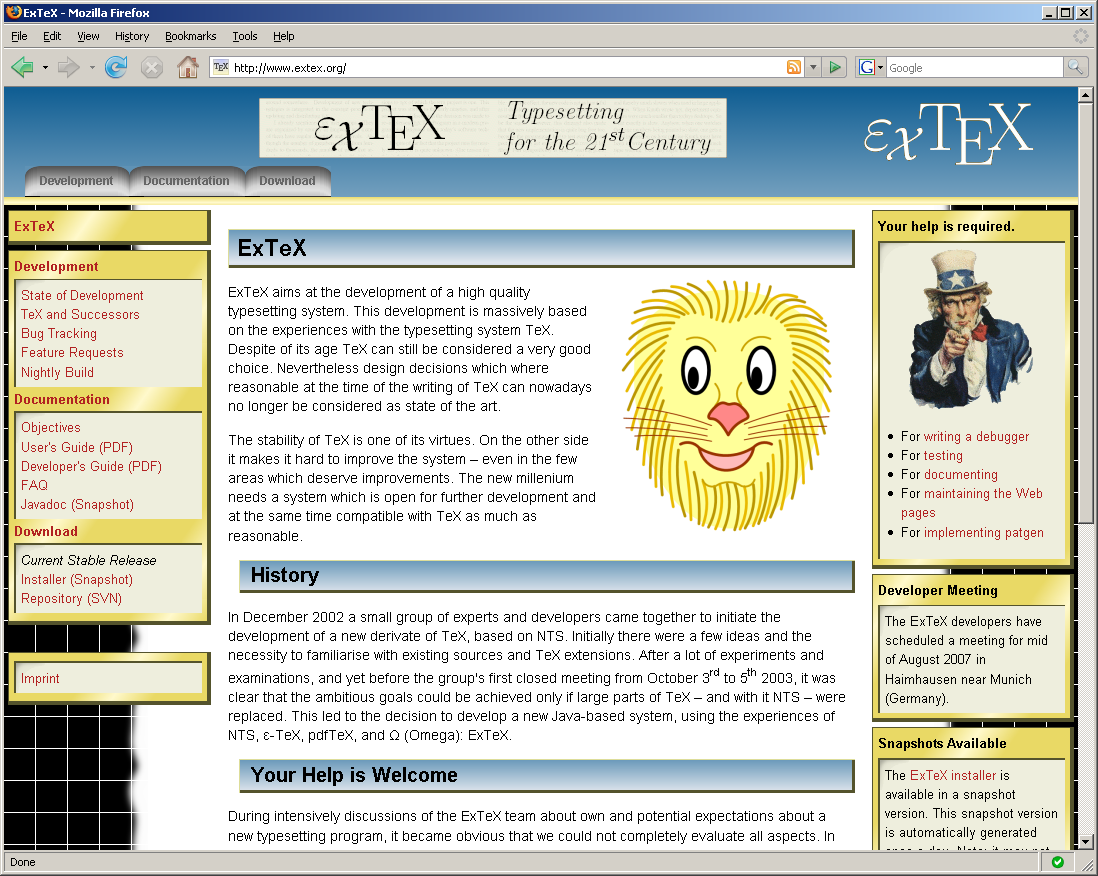
\includegraphics[width=.5\textwidth]{img/www-extex-org}
  \caption{\texttt{www.extex.org}}
  \label{fig:www.exetex.org}
\end{figure}
There is a web site devoted to \ExTeX.\index{WWW}\index{Web Site} This
web site (see figure~\ref{fig:www.exetex.org}) can be reached via the
URL\index{www.extex.org}
\begin{quotation}
  \url{http://www.extex.org}
\end{quotation}


\section{Mailing Lists}
%@author Gerd Neugebauer

If you are ready to try \ExBib{} you might as well want to join a
mailing list to get in contact with the community.\index{mailing list}

\begin{quotation}
  \url{http://www.dante.de/listman/extex}
\end{quotation}


\section{Reporting Bugs}
%@author Gerd Neugebauer


If you find any bugs in \ExBib\ you can submit them 
%either 
via a HTML form.
% or via email. 
You can find the HTML form at
\begin{quotation}
  \url{http://www.extex.org/bugs}
\end{quotation}
%Emails containing the description can be sent to
%\begin{quotation}
%  \href{mailto:extex-bugs@dante.de}{extex-bugs@dante.de}
%\end{quotation}

Please include in your description 
\begin{itemize}
\item the source of a \emph{minimal} example showing the problem
\item the log file resulting from running this example
\item a description why you think that something went wrong and what
  the expected result would be
\item a description of the environment you are using (host
  architecture, operating system, Java version)
\end{itemize}

\endinput
%
% Local Variables: 
% mode: latex
% TeX-master: "exbib-users"
% End: 


%------------------------------------------------------------------------------
\chapter{Getting Started}
%@author Gerd Neugebauer

In this chapter we describe the steps you can take to get \ExTeX\ up
and running. We try to use as few as possible premises. Thus it should
be not too hard to get started.

\section{Prerequisites}
%@author Gerd Neugebauer

\subsection{Java}
%@author Gerd Neugebauer

You need to have Java 5\index{Java} or later installed on your
system. You can get Java for a several systems directly from
\url{java.sun.com}. Download and install it according to the
installation instructions for your environment.

To check that you have an appropriate Java on your path you can use
the command \texttt{java} with the argument \texttt{-version}. This
can be seen in the following listing:

\lstset{morecomment=[l]{\#}}%
\begin{lstlisting}{morecomment=[l][keywordstyle]{>}}
# java -version
java version "1.5.0_04"
Java(TM) 2 Runtime Environment, Standard Edition (build 1.5.0_04-b05)
Java HotSpot(TM) Client VM (build 1.5.0_04-b05, mixed mode)
#
\end{lstlisting}


\subsection{TEXMF}
%@author Gerd Neugebauer

If you want to use more than the pure \ExBib\ engine, fonts and macros
can be inherited from a texmf tree\index{texmf}. \ExBib\ itself does
not contain a full texmf tree. It comes just with some rudimentary
files necessary for testing. Thus you should have installed a texmf
tree, e.g. from a \TeX Live\index{TeXlive@\TeX Live} installation.
This can be found on the \href{http://www.ctan.org}{Comprehensive
  \TeX\ Archive Network (CTAN)}\index{CTAN}.

There is no need to install the texmf tree in a special place. You
have to tell \ExBib\ anyhow where it can be found. It is even possible
to work with several texmf trees.

One requirement for the texmf trees is that they have a file database
(\File{ls-R}). \ExBib\ can be configured to work without it, but then
\ExBib\ is deadly slow. Thus you do not really want to try this
alternative.


\section{Getting \ExBib}
%@author Gerd Neugebauer

\subsection{Getting the Installer}
%@author Gerd Neugebauer

The simplest way to get \ExBib\ up and running is to use the \ExBib\ 
installer. This installer\index{installer} is distributed as one file
\File{ExBib-setup.jar}. You can download it from

\begin{quotation}
  \url{http://www.extex.org/download/}
\end{quotation}

If you have got the installer there is no need for you to get the
sources as well. Thus you can skip the following section.


\subsection{Getting the Sources}
%@author Gerd Neugebauer

The sources of \ExTeX\ are stored in a Subversion repository. To access this
repository you need access to the internet and Subversion installed in some
way.


The coordinates of the repository are:\index{repository}\index{CVS}
\medskip
\begin{quotation}
  \texttt{https://svn.berlios.de/svnroot/repos/extex}
\end{quotation}
\bigskip

We assume here that you have access to Subversion on the command line.
This can be either a shell on a Unix-like system or something like
cygwin on Windows. We also assume that you have direct connection to
the internet or Subversion configured to access the repository on the
internet.

First we create a directory where the sources are stored:
\begin{lstlisting}{}
# mkdir ExBib
\end{lstlisting}

Next we change the current directory to this base directory:
\begin{lstlisting}{}
# cd ExBib
\end{lstlisting}

Finally we can check out the sources:
\begin{lstlisting}{}
# svn checkout https://svn.berlios.de/svnroot/repos/extex/trunk/ExBib
\end{lstlisting}

This command shows a lot of output. At the end the current directory
contains the sub-directory \texttt{trunk} which is filled with a lot
of files and directories.


\section{Installing \ExBib}
%@author Gerd Neugebauer

There are several ways to install \ExBib.
The easiest installation of \ExBib\ works with the \ExBib\ installer.
This installer is named \File{ExBib-setup.jar}. You can start the
installer with the following command line:\index{installer}

\begin{lstlisting}{}
# java -jar ExTeX-setup.jar
\end{lstlisting}

On Windows\index{Windows} with a properly installed Java\index{Java}
you can also start the installer by double-clicking
\texttt{ExBib-setup.jar} in the Explorer\index{Explorer}.

\begin{figure}[t]
  \centering
  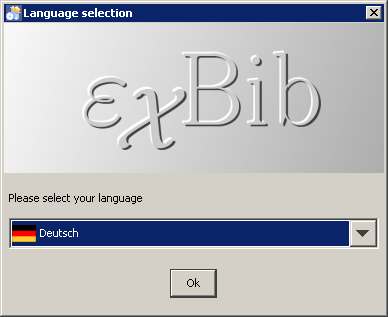
\includegraphics[width=.8\textwidth]{img/inst1}
  \caption{The Language Selection in the Installer}

  \label{fig:inst1}
\end{figure}
The installer provides a graphical user interface with a wizard
guiding you through the installation process. The first dialog is
shown in figure~\ref{fig:inst1}. As you can see you can select one of
several languages for the installation process. Currently the
languages English and German are supported. There might be some more
at the time you are performing the
installation.\index{installer!language}\index{language!installer}

Note that the internationalization covers the installer only. \ExBib\
can be run under different language environments as well. This is
controlled by a setting at run-time. Currently only an English
language binding for \ExBib\ is provided.\index{language}

Finally you have to make sure that the executables \Prog{exbib} or
\Prog{exbib.bat} is on your path for executables.\index{path}


\subsection{Replaying an Installation}
%@author Gerd Neugebauer

Sometimes it is desirable to perform an installation on several
similar machines. This means that the answers to the questions in the
installer are the same. This process can be automated.
\begin{figure}[tp]
  \centering
  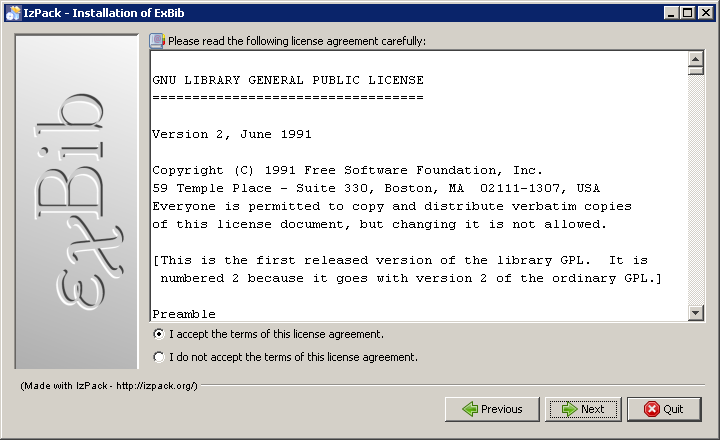
\includegraphics[width=.8\textwidth]{img/inst4}
  \caption{Generating a Auto-Configuration for the Installer}
  \label{fig:inst8}
\end{figure}

In figure~\ref{fig:inst8} you can see the last screen of the
installer. Here you have the possibility to select the button
``Generate an automatic installation script''. This produces an XML
file which can be passed to the installer to avoid the
dialogs.\index{installer}\index{installation script}

Suppose you have named the file \texttt{replay.xml} in the file
selector which pops up when the button has been pressed. Then you can
replay the installation with the following command invocation:

\begin{lstlisting}{}
# java -jar ExBib-setup.jar replay.xml
\end{lstlisting}

This supposes that the two files \File{ExTeX-setup.jar} and
\texttt{replay.xml} are in the current directory.
Finally you have to make sure that the executables \Prog{extex} or
\Prog{extex.bat} is on your path for executables.\index{path}


%------------------------------------------------------------------------------
\section{Running \ExTeX}
%@author Gerd Neugebauer

Currently \ExTeX\ can be run from the command line. In this respect it
is more or less identical to \TeX\ and can be used as a plug-in
replacement.

The following sample show a simple invocation of \ExTeX\ without any
command line arguments.

{\lstset{morecomment=[l]{*}}%
\begin{lstlisting}{}
# extex
This is ExTeX, Version 0.0 (TeX compatibility mode)
**\relax

*\end

No pages of output.
Transcript written on ./texput.log.
\end{lstlisting}}

In this case \ExTeX\ enters interaction with the user and asks for an
input file. This is indicated by the two asterisks. We have entered
\macro{relax} here to indicate that we are not willing to pass in a
file name. The \ExTeX\ system asks us to enter some command --
indicted by the single asterisk. Here we have entered \macro{end} to
indicate that we want to finish the processing. Thus \ExTeX\ 
terminates normally.

\INCOMPLETE

{\lstset{morecomment=[l]{*}}%
\begin{lstlisting}{}
# extex plain
This is ExTeX, Version 0.0 (TeX compatibility mode)
(plain Preloading the plain format: codes, registers, parameters, fonts,
more fonts, macros, math definitions, output routines, hyphenation(hyphen))
*\dump
Beginning to dump on file plain.fmt

*\end

No pages of output.
Transcript written on ./plain.log.
\end{lstlisting}}


\subsection{Command Line Parameters}
%@author Gerd Neugebauer

The invocation of the executable \Prog{extex} can be controlled by
large number of command line arguments. Those command line arguments
are described in the following list:

\begin{description}
\item[\Arg{code}]\ \\
  This parameter contains \ExTeX\ code to be executed directly. The
  execution is performed after any code specified in an input file. On
  the command line the code has to start with a backslash. This
  restriction does not hold for the property settings.

  This command line argument sets the property \Property{extex.code}
  
\item[\Arg{file}]\ \\
  This parameter contains the file to read from. A file name may not
  start with a backslash or an ambercent. It has no default.

  This command line argument sets the property \Property{extex.file}.
  
\item[\CLI{-} \Arg{file}]\ \\
  This parameter terminates the normal processing of arguments. The
  next argument -- if present -- is interpreted as input file. With
  this construction it is possible to process an input file which
  starts with one of the special characters \verb|\| or \verb|&|.

  This command line argument sets the property \Property{extex.file}
  if a file argument is present.

\item[\CLI{configuration} \Arg{resource}]\ \\
  This parameter contains the name of the configuration resource to
  use. This configuration resource is sought on the class path.
  
  This command line argument sets the property \Property{extex.config}.
  
\item[\CLI{copyright}]\ \\
  This command line option produces a copyright notice on the standard
  output stream and terminates the program afterwards.

\item[\tt\&\Arg{format}]\index{\&}
\item[\CLI{fmt} \Arg{format}]\ \\
  This parameter contains the name of the format to read. An empty
  string denotes that no format should be read. This is the default.

  This command line argument sets the property \Property{extex.format}.
  
\item[\CLI{debug} \Arg{spec}]\ \\
  This command line parameter can be used to instruct the program to
  produce debugging output of several kinds. The debug output is
  written to the log file. The specification \Arg{spec} is interpreted
  left to right. Each character is interpreted according to the
  following table:

  \begin{tabular}{lp{.4\textwidth}l}\toprule
    \textit{Spec}& \textit{Description}& \textit{See} \\\midrule
    F& 	This specifier contains the indicator whether or not to trace
    the searching for input files. & 	\Property{extex.trace.input.files}\\
    f& 	This specifier contains the indicator whether or not to trace
    the searching for font files.&      \Property{extex.trace.font.files}\\
    M& 	This specifier contains the indicator whether or not to trace
    the execution of macros.&	 	\Property{extex.trace.macros}\\
    T& 	This specifier contains the indicator whether or not to trace
    the work of the tokenizer.& 	\Property{extex.trace.tokenizer}\\
    \bottomrule
  \end{tabular}

  The following example shows a possible invocation with this
  parameter: 
\begin{lstlisting}{}
# extex -debug FfMT abc.tex
This is ExTeX, Version 0.0 (TeX compatibility mode)
...
\end{lstlisting}
  
\item[\CLI{halt-on-error}]\ \\
  This parameter contains the indicator whether the processing should
  halt after the first error which has been encountered.

  This command line argument sets the property \Property{extex.halt.on.error}.
  
\item[\CLI{help}]\ \\
  This command line option produces a short usage description on the
  standard output stream and terminates the program afterwards.
  
\item[\CLI{ini}]\ \\
  If set to true then act as ini\TeX.\index{initex@ini\TeX} In this
  case no format has to be preloaded. All parameters are set to the
  "`factory settings"'.

  This command line argument sets the property \Property{extex.ini}.

  The following example shows a possible invocation with this
  parameter: 
\begin{lstlisting}{}
# extex -ini abc.tex
This is ExTeX, Version 0.0 (TeX compatibility mode)
...
\end{lstlisting}
  
\item[\CLI{interaction} \Arg{mode}]\ \\
  This parameter contains the interaction mode. possible values are
  the numbers 0\dots3 and the symbolic names \Mode{batchmode} (0),
  \Mode{nonstopmode} (1), \Mode{scrollmode} (2), and
  \Mode{errorstopmode} (3).

  This command line argument sets the property \Property{extex.interaction}.
  
  The following example shows a possible invocation with this
  parameter:
\begin{lstlisting}{}
# extex -interaction batchmode abc.tex
This is ExTeX, Version 0.0 (TeX compatibility mode)
...
\end{lstlisting}

\item[\CLI{job-name} \Arg{name}]\ \\
  This parameter contains the name of the job. It is overwritten if a
  file is given to read from. In this case the base name of the input
  file is used instead.

  This command line argument sets the property \Property{extex.jobname}.
  
\item[\CLI{language} \Arg{language}]\ \\
  This parameter contains the name of the locale to be used for the
  messages.

  This command line argument sets the property \Property{extex.lang}.
  
\item[\CLI{output} \Arg{format}]\ \\
  This parameter contains the output format. This logical name is
  resolved via the configuration.

  This command line argument sets the property \Property{extex.output}.

  The following example shows a possible invocation with this
  parameter: 
\begin{lstlisting}{}
# extex -output pdf abc.tex
This is ExTeX, Version 0.0 (TeX compatibility mode)
\end{lstlisting}
  
\item[\CLI{progname} \Arg{name}]\ \\
  This parameter can be used to overrule the name of the program shown
  in the banner and the version information.  The following example
  shows a possible invocation and the resulting output:

\begin{lstlisting}{}
# extex -progname XeTxE -version
This is XeTxE, Version 0.0 (1.4.2_06)
#
\end{lstlisting}

  This command line argument sets the property \Property{extex.progname}.
  
\item[\CLI{texinputs} \Arg{path}]\ \\
  This parameter contains the additional directories for searching
  \ExTeX\ input files.  The directories are separated by the
  system-dependant separator.  This separator is a colon (\verb|:|) on
  Unix\index{Unix} and the semicolon (\verb|;|) on
  Windows\index{Windows}.
  
  This command line argument sets the property
  \Property{extex.texinputs}.
  
\item[\CLI{texmfoutputs} \Arg{dir}]\ \\
  This parameter contains the name of the property for the fallback if
  the output directory fails to be writable.
  
  This command line argument sets the property
  \Property{extex.outputdir.fallback}.
  
\item[\CLI{texoutputs} \Arg{dir}]\ \\
  This parameter contain the directory where output files should be
  created.

  This command line argument sets the property \Property{extex.outputdir}.
  
\item[\CLI{version}]\ \\
  This command line parameter forces that the version information is
  written to standard output and the program is
  terminated.\index{version} The version of \ExTeX\ is shown and the
  version of the Java engine\index{Java} in parentheses. The following
  example shows a possible invocation and the resulting output:

\begin{lstlisting}{}
# extex -version
This is ExTeX, Version 0.0 (1.4.2_06)
#
\end{lstlisting}
\end{description}

Command line parameters can be abbreviated up to a unique prefix --
and sometimes even more. Thus the following invocations are
equivalent:

\begin{verbatim}
  extex -v
  extex -ve
  extex -ver
  extex -vers
  extex -versi
  extex -versio
  extex -version  
\end{verbatim}


\begin{DirList}{200pt}{250pt}
  \TOPDIR(0,30){ExBib}
  \DIR(3,28)2{Uninstaller}
  \FILE(6,26)2{uninstaller.jar}
  \DIR(3,24){4.75}{bin}
  \FILE(6,22)2{exbib}
  \FILE(6,20){2.5}{exbib.bat}
  \FILE(6,18){2.5}{exbibutil}
  \FILE(6,16){2.5}{exbibutil.bat}
  \DIR(3,14){10.75}{doc}
  \FILE(6,12)2{exbib-users.pdf}
  \DIR(3,10){4.75}{lib}
  \FILE(6,8){2}{ExBib-core.jar}
  \FILE(6,6){2.5}{ExBib-Main.jar}
  \FILE(6,4){2.5}{ExBib-styles.jar}
  \FILE(6,2){2.5}{ExTeX-resource.jar}
  \FILE(3,0){10.75}{LICENSE.txt}
\end{DirList}


%%*****************************************************************************
%% $Id$
%%*****************************************************************************
%% Author: Gerd Neugebauer
%%-----------------------------------------------------------------------------

\chapter{The Data Base}


\section{Syntax}

The data base in \BibTeX\index{BibTeX@\BibTeX} style consists of a
simple text file. \IM{08x1}

The following characters have a special meaning for the \BibTeX\
syntax:
\begin{verbatim}
    @ { } ( ) , # " =
\end{verbatim}
Any other character is treated equally as ordinary character.

An instruction is started with an at sign (@) followed by its name.
The name is composed of upper or lowercase letters and digits.

Whatever follows the name of the instruction depends on the
instruction. In most cases the parameters for the instruction are
following. They are enclosed in braces. For compatibility with
Scribe\index{Scribe} parentheses are sometimes allowed instead of the
braces.


\section{The \texttt{@input} Instruction}%
\index{@input|(}

Sometimes it might be desirable to split a database into several
segements. This is supported by the ability to pass inseveral
databases via the aux file. The \texttt{@input} instruction provides
another mechanism for the same which acts on the level of the database
files. \IM{x1}

The instruction takes as argument a resource name. It includes the
content as if it where present at the place of the instruction.

\begin{lstlisting}[language=bibtex,alsoletter={@},morekeywords={@input}]
  @input(some/other/resource)
\end{lstlisting}

The formal syntax of this instruction is as follows:
\begin{syntax}
  \tag{instruction}\SyntaxDef \texttt{@input} \texttt{\char`\{}
                                \tag{resource name} \texttt{\char`\}}
\end{syntax}%
\index{@input|)}


\section{Entries}

Any instruction which has no special meaning is considered to be an
entry in the database.
\IM{08x1}


\begin{lstlisting}[language=bibtex]
  @Book{          knuth:texbook,
    author      = {Donald E. Knuth},
    title       = {The {\TeX book}},
    publisher   = {Addison-Wesley Publishing Company},
    address     = {Reading, Mass.},
    year        = 1989,
    edition     = {15},
    volume      = {A},
    series      = {Computers and Typesetting}
  }
\end{lstlisting}

\INCOMPLETE

The formal syntax of this instruction is as follows:
\begin{syntax}
  \tag{instruction} \SyntaxDef \texttt{@} \tag{type} \texttt{\char`\{}
                      \tag{key} \texttt{,} \tag{attributes} \texttt{\char`\}} \\
                    \SyntaxOr  \texttt{@} \tag{type} \texttt{(}
                      \tag{key} \texttt{,} \tag{attributes} \texttt{)}\\
  \tag{attributes}  \SyntaxDef \tag{attribute}\\
                    \SyntaxOr  \tag{attribute} \texttt{,} \tag{attributes}\\
  \tag{attribute}   \SyntaxDef \tag{field name} \texttt{=} \tag{value}\\
  \tag{value}       \SyntaxDef \tag{atomic value}\\
                    \SyntaxOr  \tag{atomic value} \texttt{\#} \tag{value}\\
  \tag{atomic value}\SyntaxDef \texttt{"} \tag{string} \texttt{"}\\
                    \SyntaxOr  \texttt{\char`\{} \tag{block} \texttt{\char`\}}\\
                    \SyntaxOr  \tag{number}\\
                    \SyntaxOr  \tag{macro name}
\end{syntax}%
Several syntactic entities deserve a definition:

\begin{description}
\item[\tag{type}] \ \\
  A \tag{type} is a non-empty sequence of characters which is not one
  of the special characters or white-space. The type is considered
  case insensitive; i.e. upper and lowercase letters are considered
  the same.
\item[\tag{key}] \ \\
  A \tag{key} is a non-empty sequence of characters which is not one
  of the special characters or white-space. The type is considered
  case insensitive.
\item[\tag{field name}] \ \\
  A \tag{field name} is a non-empty sequence of characters which is
  not one of the special characters or white-space. The type is
  considered case insensitive.
\item[\tag{string}] \ \\
  A \tag{string} is a sequence of characters with balenced braces
  which does not contain a double quote \verb|"| at brace level 0.
\item[\tag{block}] \ \\
  A \tag{block} is a sequence of characters with balanced braces; The
  braces preceded by a backslash do not count for balancing.
\item[\tag{number}] \ \\
  A \tag{number} is a not empty sequence of digits.
\item[\tag{macro name}] \ \\
  A \tag{macro name} is a non-empty sequence of characters which is
  not one of the special characters or white-space. The type is
  considered case insensitive.
\end{description}


\section{Names}\label{sec:names}%
\index{name|(}

Names are especially complicated and deserve a description of their
own. 
\IM{08x1}

\subsection{Name Components}

\BibTeX\ uses four components for names. Any name is analyzed and
decomposed into the four parts. The following parts of names are
considered:

\begin{description}
\item[Last part] \ \\
  The last name or christian name of a person is usually the last
  major component of a name. This is the only part which is not
  optional.
\item[First parts] \ \\
  The first name or given name of a person is usually the first
  component of a name. This part is optional.
\item[Von part] \ \\
  The von part of a name usually comes between first name and last
  name and starts with lowercase letters. It is optional.
\item[Junior part] \ \\
  The junior part of a name is an addition appended to the name. This
  part is optional.
\end{description}

The parts are separated by white space. This whitespace is only
consoidered if it occurs at brace level 0. Thus the grouping with
braces is honored. It can be used to tie together parts which would be
torn apart otherwise.

Any part can consist of several words. Commas can be used to structure
a name. Thus we will use the number of commas for the analysis as
well.
\def\First#1{#1}%
\def\Last#1{\textbf{#1}}%
\def\Von#1{\textit{#1}}%
\def\Jr#1{\underline{#1}}%

\subsubsection*{No Commas}

If a name does not contain a comma then the following pattern is used
to determine the parts of the name:

\begin{syntax}
  \tag{name}\SyntaxDef\tag{first}* \tag{von}* \tag{last} \tag{jr}* 
\end{syntax}%
The name parts \emph{first} and \emph{last} consit of words for which
the first letter is an uppercase letter. The name parts \emph{von} and
\emph{jr} consit of words for which the first letter is a lowercase
letter.

The following examples show who teh names are classified. The last
name is printed in bold, the first name is printed in roman, the von
part is printed in italics and the junior part is underlined.

\begin{quote}\obeylines
  \Last{Aristoteles}
  \First{Leslie} \Last{Lamport}
  \First{Donald Ervin} \Last{Knuth}
  \First{Johannes Chrysostomus Wolfgangus Theophilus} \Last{Mozart}
  \First{Ludwig} \Von{van} \Last{Beethoven}
  \First{Otto Eduard Leopold} \Von{von} \Last{Bismarck-Sch�nhausen}
  \First{Miguel} \Von{de} \Last{Cervantes Saavedra}
  \First{Sammy} \Last{Davis} \Jr{jr.}
  \First{Don Quixote} \Von{de la} \Last{Mancha}
\end{quote}


\subsubsection*{One Comma}

If a name does not contain a comma then the following pattern is used
to determine the parts of the name:

\begin{syntax}
  \tag{name}\SyntaxDef \tag{von}* \tag{last} \texttt{,} \tag{first}* \\
            \SyntaxOr  \tag{first}* \tag{von}* \tag{last} \texttt{,} \tag{jr}* 
\end{syntax}%
The name parts \emph{first} and \emph{last} consit of words for which
the first letter is an uppercase letter. The name parts \emph{von} and
\emph{jr} consit of words for which the first letter is a lowercase
letter.

The following examples show who teh names are classified. The last
name is printed in bold, the first name is printed in roman, the von
part is printed in italics and the junior part is underlined.

\begin{quote}\obeylines
  \Last{Lamport}, \First{Leslie}
  \Last{Knuth}, \First{Donald Ervin} 
  \Last{Mozart}, \First{Johannes Chrysostomus Wolfgangus Theophilus} 
  \Last{Beethoven}, \First{Ludwig} \Von{van} 
  \Von{von} \Last{Bismarck-Sch�nhausen}, \First{Otto Eduard Leopold} 
  \Von{de} \Last{Cervantes Saavedra}, \First{Miguel} 
  \First{Sammy} \Last{Davis}, \Jr{Jr.}
\end{quote}


\subsubsection*{Two Commas}

If a name does not contain a comma then the following pattern is used
to determine the parts of the name:

\begin{syntax}
  \tag{name}\SyntaxDef \tag{von}* \tag{last} \texttt{,} \tag{first}* \\
            \SyntaxOr  \tag{last} \tag{von}* \texttt{,} \tag{jr}
            \texttt{,} \tag{first}* 
\end{syntax}%
The name parts \emph{first} and \emph{last} consit of words for which
the first letter is an uppercase letter. The name parts \emph{von} and
\emph{jr} consit of words for which the first letter is a lowercase
letter.

The following examples show who teh names are classified. The last
name is printed in bold, the first name is printed in roman, the von
part is printed in italics and the junior part is underlined.

\begin{quote}\obeylines
  \Last{Davis}, \First{Sammy}, \Jr{Jr.}
\end{quote}


\subsubsection*{More Commas}

More than two commas are not understood by the name parsing in \ExBib.


\subsection{Name Lists}
\index{name list|(}

Names usually come in bibliographies as single names or as lists of
names. Thus we have to take care of lists of names. Those lists are
made up of single names separated by the word \texttt{and} surrounded
by whitespace. This separator is only considered at brace level 0.
Thus it is possible to protect embedded words ``and''. Those might be
parts of company names -- e.g. acting an author.

The following example is recognizes as two names:
\begin{quote}\obeylines
  \Last{Barnes} and \Last{Noble}
\end{quote}
The following example is recognizes a a single name name:
\begin{quote}\obeylines
  \Last{\char`\{ Barnes and Noble\char`\}}
\end{quote}
\index{name list|)}%
\index{name|)}


\section{Comments}

Anything outside of entries and other declarations are considered as a
comment -- and mainly ignored. Thus you can put anything in between
the entries.
\IM{081}

There is one special tag to mark comments. It is the tag
\texttt{@comment}. Since anything outside of declarations is already a
comment. Is has been considered sufficient to ignore the tag in the
input stream.
\begin{lstlisting}[language=bibtex]
  @comment
\end{lstlisting}

Unfortunately in the age of internet it is desirable to include email
addresses into comment -- and those may contain an @. Thus the
definition of the \texttt{@comment} declaration is slightly different
from \BibTeX\index{BibTeX@\BibTeX}:
\IM{x}
\begin{itemize}
\item If the next non-space character is an opening brace (\verb|{|)
  then a block is read and treated as comment. This means that the
  block can contain arbitrary characters -- especially the @ sign.
  On the other side the block needs to have balanced braces.
\begin{lstlisting}[language=bibtex]
  @comment{ This is a comment with embedded @ }
\end{lstlisting}
    
\item If the next non-space character is not an open brace character
  then just the tag is ignored.
\begin{lstlisting}[language=bibtex]
  @comment This is a comment
\end{lstlisting}
  
\end{itemize}


\section{The \texttt{@alias} Instruction}%
\index{@alias|(}

The \texttt{@alias} instruction can be used to define alternative keys
for an entry. Whenever an entry is references with one of its keys all
aliases are considered to be the same. For instance when an entry has
two keys defined via the \texttt{@alias} and both of them are uned in
a \macro{cite} then it is included in the result list only once.
\IM{x1}

\begin{lstlisting}[language=bibtex]
  @alias( abc = def )
\end{lstlisting}

To define an alias give the new key followed by an equality sign and
the old key as argument to the \texttt{@alias} instruction. The enty
for the old key has to exist at the time the \texttt{@alias}
instruction is encountered.

The formal syntax of this instruction is as follows:
\begin{syntax}
  \tag{instruction}\SyntaxDef \texttt{@alias} \texttt{\char`\{}
                     \tag{key1} \texttt{=} \tag{key2} \texttt{\char`\}}\\
                   \SyntaxDef \texttt{@alias} \texttt{(}
                     \tag{key1} \texttt{=} \tag{key2} \texttt{)}
\end{syntax}%
The instruction name is compared case insensitive.
\index{@alias|)}

\section{The \texttt{@modify} Instruction}%
\index{@modify|(}

The \texttt{@modify} instruction can be used to alter the content of
certain fields in an entry. The question is why would such a directive
be necessary when you could simply alter the entry itself. The answer
is that the entry might not be under your control. It might be
contained in another file which is included via the \texttt{@include}
directive.
\IM{x1}

\begin{lstlisting}[language=bibtex]
  @modify( abc,
           author = {A.U. Thor} )
\end{lstlisting}

The argument of the \texttt{@modify} instruction looks formally like
the argument for an entry. Instead of specifying a new entry an
existing entry with the given key is sought and the given field values
are overwritten. If no entry corresponding to the given key can be
found then an error is raised.


The formal syntax of this instruction is as follows:
\begin{syntax}
  \tag{instruction}\SyntaxDef \texttt{@modify} \texttt{\char`\{}
                     \tag{key} \texttt{,} \tag{attributes} \texttt{\char`\}}\\
                   \SyntaxDef \texttt{@alias} \texttt{(}
                     \tag{key} \texttt{,} \tag{attributes} \texttt{)}
\end{syntax}%
The instruction name is compared case insensitive.
\index{@modify|)}


\section{The \texttt{@string} Instruction}%
\index{@string|(}

The \texttt{@string} instruction can be used to define macros. Each
macro has a name and a value. When a field of an entry is accessed the
field value is computed. The computation concatenats its parts. In
this course the macros contained are resolved.
\IM{08x1}

The macros can be defined in several places. One of them is the
datatebase file. Another is the style file. The place where the
definition is located does not make a difference.

\begin{lstlisting}[language=bibtex]
  @string( abc = {The value} )
\end{lstlisting}

The formal syntax of this instruction is as follows:
\begin{syntax}
  \tag{instruction}\SyntaxDef \texttt{@string} \texttt{\char`\{}
                     \tag{macro name} \texttt{=} \tag{value} \texttt{\char`\}}\\
                   \SyntaxDef \texttt{@string} \texttt{(}
                     \tag{macro name} \texttt{=} \tag{value} \texttt{)}
\end{syntax}%
The instruction name is compared case in-sensitove.
\index{@string|)}


\section{The \texttt{@preamble} Instruction}
\index{@preamble|(}

Sometines it is necessary ensure that a certain definition is made
which is used in the database. Those definitions are collected and can
be included at the beginning of the generated output.
\IM{08x1}

\begin{lstlisting}[language=bibtex]
  @preamble( "\providecommand\BibTeX{\textsc{Bib}\TeX}" )
\end{lstlisting}

The formal syntax of this instruction is as follows:
\begin{syntax}
  \tag{instruction}\SyntaxDef \texttt{@preamble} \texttt{\char`\{}
                     \tag{value} \texttt{\char`\}}\\
                   \SyntaxDef \texttt{@preamble} \texttt{(}
                     \tag{value} \texttt{)}
\end{syntax}%
The instruction name is compared case in-sensitove.
\index{@preamble|(}

\endinput
%
% Local Variables: 
% mode: latex
% TeX-master: "../exbib-manual"
% End: 

%%*****************************************************************************
%% $Id: bst-language.tex,v 0.00 2008/04/30 23:26:21 gene Exp $
%%*****************************************************************************
%% Author: Gerd Neugebauer
%%-----------------------------------------------------------------------------

\chapter{The Styles}

\BibTeX~0.99c\index{BibTeX 0.99c@\BibTeX~0.99c} is accompanied by some
style files. They can be used out of the box. They are contained in
\ExBib\ as well. They are described here.

\section{plain}
\index{bst!plain|(}
\INCOMPLETE
\index{bst!plain|)}

\section{alpha}
\index{bst!alpha|(}
\INCOMPLETE
\index{bst!alpha|)}

\section{unsrt}
\index{bst!unsrt|(}
\INCOMPLETE
\index{bst!unsrt|)}

\section{abbrev}
\index{bst!abbrev|(}
\INCOMPLETE
\index{bst!abbrev|)}


\endinput
%
% Local Variables: 
% mode: latex
% TeX-master: "../exbib-manual"
% End: 

%%*****************************************************************************
%% $Id: bst-language.tex,v 0.00 2008/04/30 23:26:21 gene Exp $
%%*****************************************************************************
%% Author: Gerd Neugebauer
%%-----------------------------------------------------------------------------

\chapter{Tools}

\section{The \ExBib\ Util}

\subsection{Command Line Arguments}


\INCOMPLETE


\endinput
%
% Local Variables: 
% mode: latex
% TeX-master: "../exbib-manual"
% End: 
the Style
%%*****************************************************************************
%% $Id: bst-language.tex,v 0.00 2008/04/30 23:26:21 gene Exp $
%%*****************************************************************************
%% Author: Gerd Neugebauer
%%-----------------------------------------------------------------------------

\chapter{The BST Language}%
\index{BST language|(}

\IM{08x1}%
The processing of the data base entries can be programmed with a small
special purpose programming language. Since it seems to have no name
it is called the BST language

Usually the instructions are read from a file. The default extension
of these files is \texttt{.bst}. The content is interpreted to produce
the formatted output.

The primary goal of \BibTeX\index{BibTeX@\BibTeX} is the processing of
bibliographic databases. Thus the language is tailored towards the
formatting of bibliographies.


\def\cmdIndex#1{\index{#1@\texttt{#1}}}%
\def\fctIndex#1{\index{#1@\texttt{#1}}%
  \index{function!#1@\texttt{#1}}}%
\def\varIndex#1{\index{#1@\texttt{#1}}%
  \index{variable!#1@\texttt{#1}}}%

\section{The Programming Model}

The BST language is based on a simple stack based metaphor. The stack
is the central data structure in the program. The stack is able to
carry arbitrary data. Especially it is possible to push code segments
to the stack.

\begin{figure}[tb]
  \centering
  %%*****************************************************************************
%% Copyright (c) 2008 Gerd Neugebauer
%%
%% Permission is granted to copy, distribute and/or modify this document
%% under the terms of the GNU Free Documentation License, Version 1.2
%% or any later version published by the Free Software Foundation;
%% with no Invariant Sections, no Front-Cover Texts, and no Back-Cover Texts.
%%
%%*****************************************************************************
%% $Id:bst-model.tex 7067 2008-05-18 11:06:56Z gene $
%%*****************************************************************************
%% Author: Gerd Neugebauer
%%-----------------------------------------------------------------------------
\begingroup
\begin{tikzpicture}[scale=.7]\sf\bfseries
  % --- bottom layer ---
  \shade[top color=white!97!blue,bottom color=white!90!blue,draw=blue!40!black,thick]
  (0,0) rectangle (15,10);
  \draw[fill=gray!20!white] (0,10) -- (.1,10.1) -- (15.1,10.1) -- (15,10) -- cycle;
  \draw[fill=gray!20!white] (15,10) -- (15.1,10.1) -- (15.1,.1) -- (15,0) -- cycle;

  % --- code ---
  \begin{scope}[shift={(6.25,9.5)},scale=.5]
    \begin{scope}[shift={(.5,.5)}]
      \shade[top color=white!90!yellow,bottom color=white!60!yellow,draw=red!40!black,thick]
      (0,0) -- (5,0) -- (5,2) -- (4,3) -- (0,3) -- cycle;
    \end{scope}
    \begin{scope}[shift={(.4,.4)}]
      \shade[top color=white!90!yellow,bottom color=white!60!yellow,draw=red!40!black,thick]
      (0,0) -- (5,0) -- (5,2) -- (4,3) -- (0,3) -- cycle;
    \end{scope}
    \begin{scope}[shift={(.3,.3)}]
      \shade[top color=white!90!yellow,bottom color=white!60!yellow,draw=red!40!black,thick]
      (0,0) -- (5,0) -- (5,2) -- (4,3) -- (0,3) -- cycle;
    \end{scope}
    \begin{scope}[shift={(.2,.2)}]
      \shade[top color=white!90!yellow,bottom color=white!60!yellow,draw=red!40!black,thick]
      (0,0) -- (5,0) -- (5,2) -- (4,3) -- (0,3) -- cycle;
    \end{scope}
    \begin{scope}[shift={(.1,.1)}]
      \shade[top color=white!90!yellow,bottom color=white!60!yellow,draw=red!40!black,thick]
      (0,0) -- (5,0) -- (5,2) -- (4,3) -- (0,3) -- cycle;
    \end{scope}
    \shade[top color=white!90!yellow,bottom color=white!60!yellow,draw=red!40!black,thick]
    (0,0) -- (5,0) -- (5,2) -- (4,3) -- (0,3) -- cycle;
  \end{scope}
  \draw (7.5,10.25) node {Code};

  % --- interpreter ---
  \shade[top color=white!90!blue,bottom color=white!60!blue,draw=blue!40!black,thick]
  (5,1) rectangle (10,9);
  \draw[fill=gray!20!white] (5,9) -- (5.1,9.1) -- (10.1,9.1) -- (10,9) -- cycle;
  \draw[fill=gray!20!white] (10,9) -- (10.1,9.1) -- (10.1,1.1) -- (10,1) -- cycle;
  \draw (7.5,5) node {Interpreter};
  
  \shade[top color=white!90!green,bottom color=white!60!green,draw=green!40!black,thick]
  (5,-.5) .. controls (6,0) and (9,-1) .. (10,-.5) -- (10,.5) -- (5,.5) -- cycle;
  \draw (7.5,0) node {Output Stream};


  % --- stack ---
  \shade[top color=white!10!pink,bottom color=white!90!pink,draw=pink!70!black,shift={(11.5,1)}] (0,0) -- (.5,1) -- (2.5,1) -- (2,0) -- cycle;
  \shade[top color=white!10!pink,bottom color=white!90!pink,draw=pink!70!black,shift={(11.5,1.5)}] (0,0) -- (.5,1) -- (2.5,1) -- (2,0) -- cycle;
  \shade[top color=white!10!pink,bottom color=white!90!pink,draw=pink!70!black,shift={(11.5,2)}] (0,0) -- (.5,1) -- (2.5,1) -- (2,0) -- cycle;
  \shade[top color=white!10!pink,bottom color=white!90!pink,draw=pink!70!black,shift={(11.5,2.5)}] (0,0) -- (.5,1) -- (2.5,1) -- (2,0) -- cycle;
  \shade[top color=white!10!pink,bottom color=white!90!pink,draw=pink!70!black,shift={(11.5,3)}] (0,0) -- (.5,1) -- (2.5,1) -- (2,0) -- cycle;
  \shade[top color=white!10!pink,bottom color=white!90!pink,draw=pink!70!black,shift={(11.5,3.5)}] (0,0) -- (.5,1) -- (2.5,1) -- (2,0) -- cycle;
  \shade[top color=white!10!pink,bottom color=white!90!pink,draw=pink!70!black,shift={(11.5,4)}] (0,0) -- (.5,1) -- (2.5,1) -- (2,0) -- cycle;
  \shade[top color=white!10!pink,bottom color=white!90!pink,draw=pink!70!black,shift={(11.5,4.5)}] (0,0) -- (.5,1) -- (2.5,1) -- (2,0) -- cycle;
  \shade[top color=white!10!pink,bottom color=white!90!pink,draw=pink!70!black,shift={(11.5,5)}] (0,0) -- (.5,1) -- (2.5,1) -- (2,0) -- cycle;
  \shade[top color=white!10!pink,bottom color=white!90!pink,draw=pink!70!black,shift={(11.5,5.5)}] (0,0) -- (.5,1) -- (2.5,1) -- (2,0) -- cycle;
  \shade[top color=white!10!pink,bottom color=white!90!pink,draw=pink!70!black,shift={(11.5,6)}] (0,0) -- (.5,1) -- (2.5,1) -- (2,0) -- cycle;
  \shade[top color=white!10!pink,bottom color=white!90!pink,draw=pink!70!black,shift={(11.5,6.5)}] (0,0) -- (.5,1) -- (2.5,1) -- (2,0) -- cycle;
  \shade[top color=white!10!pink,bottom color=white!90!pink,draw=pink!70!black,shift={(11.5,7)}] (0,0) -- (.5,1) -- (2.5,1) -- (2,0) -- cycle;
  \shade[top color=white!10!pink,bottom color=white!90!pink,draw=pink!70!black,shift={(11.5,7.5)}] (0,0) -- (.5,1) -- (2.5,1) -- (2,0) -- cycle;
  \shade[top color=white!10!pink,bottom color=white!90!pink,draw=pink!70!black,shift={(11.5,8)}] (0,0) -- (.5,1) -- (2.5,1) -- (2,0) -- cycle;
  \draw (12.75,8.5) node {Stack};

  % --- integers ---
  \shade[top color=white!90!pink,bottom color=white!10!pink,draw=pink!70!black]
  (1,7) rectangle (4,7.4);
  \shade[shift={(0,.4)},top color=white!90!pink,bottom color=white!10!pink,draw=pink!70!black]
  (1,7) rectangle (4,7.4);
  \shade[shift={(0,.8)},top color=white!90!pink,bottom color=white!10!pink,draw=pink!70!black]
  (1,7) rectangle (4,7.4);
  \shade[shift={(0,1.2)},top color=white!90!pink,bottom color=white!10!pink,draw=pink!70!black]
  (1,7) rectangle (4,7.4);
  \shade[shift={(0,1.6)},top color=white!90!pink,bottom color=white!10!pink,draw=pink!70!black]
  (1,7) rectangle (4,7.4);
  \draw (1,7) rectangle (4,9);
  \draw (2.5,8) node {Integers};

  % --- strings ---
  \shade[top color=white!90!pink,bottom color=white!10!pink,draw=pink!70!black]
  (1,4) rectangle (4,4.4);
  \shade[shift={(0,.4)},top color=white!90!pink,bottom color=white!10!pink,draw=pink!70!black]
  (1,4) rectangle (4,4.4);
  \shade[shift={(0,.8)},top color=white!90!pink,bottom color=white!10!pink,draw=pink!70!black]
  (1,4) rectangle (4,4.4);
  \shade[shift={(0,1.2)},top color=white!90!pink,bottom color=white!10!pink,draw=pink!70!black]
  (1,4) rectangle (4,4.4);
  \shade[shift={(0,1.6)},top color=white!90!pink,bottom color=white!10!pink,draw=pink!70!black]
  (1,4) rectangle (4,4.4);
  \draw (1,4) rectangle (4,6);
  \draw (2.5,5) node {Strings};

  % --- entries ---
  \shade[top color=white!90!pink,bottom color=white!10!pink,draw=pink!70!black]
  (1,1) rectangle (4,1.4);
  \shade[shift={(0,.4)},top color=white!90!pink,bottom color=white!10!pink,draw=pink!70!black]
  (1,1) rectangle (4,1.4);
  \shade[shift={(0,.8)},top color=white!90!pink,bottom color=white!10!pink,draw=pink!70!black]
  (1,1) rectangle (4,1.4);
  \shade[shift={(0,1.2)},top color=white!90!pink,bottom color=white!10!pink,draw=pink!70!black]
  (1,1) rectangle (4,1.4);
  \shade[shift={(0,1.6)},top color=white!90!pink,bottom color=white!10!pink,draw=pink!70!black]
  (1,1) rectangle (4,1.4);
  \draw[shift={(.3,0)},draw=pink!70!black] (1,1) -- (1,3);
  \draw[shift={(.6,0)},draw=pink!70!black] (1,1) -- (1,3);
  \draw[shift={(.9,0)},draw=pink!70!black] (1,1) -- (1,3);
  \draw[shift={(1.2,0)},draw=pink!70!black] (1,1) -- (1,3);
  \draw[shift={(1.5,0)},draw=pink!70!black] (1,1) -- (1,3);
  \draw[shift={(1.8,0)},draw=pink!70!black] (1,1) -- (1,3);
  \draw[shift={(2.1,0)},draw=pink!70!black] (1,1) -- (1,3);
  \draw[shift={(2.4,0)},draw=pink!70!black] (1,1) -- (1,3);
  \draw[shift={(2.7,0)},draw=pink!70!black] (1,1) -- (1,3);
  \draw (1,1) rectangle (4,3);
  \draw (2.5,2) node {Entries};

  \begin{scope}[shift={(-5,0)}]
    \shade[left color=white!96!blue!70!pink,right color=white!60!blue!60!pink,draw=pink!70!black]
    (0,0)   .. controls (0,-.4) and (1.5,-.5) ..
    (2,-.5)  .. controls (2.5,-.5) and (4,-.4) ..
    (4,0) -- (4,4) -- (0,4) -- cycle;
    \draw[shift={(0,4)},fill=white!96!blue!70!pink,draw=pink!60!black]
    (0,0)   .. controls (0,.4) and (1.5,.5) ..
    (2,.5)  .. controls (2.5,.5) and (4,.4) ..
    (4,0)   .. controls (4,-.4) and (2.5,-.5) ..
    (2,-.5) .. controls (1.5,-.5) and (0,-.4) ..
    (0,0);
  \end{scope}
  \draw (-3,2) node {Database};

%  \draw[shift={(0,-5)}]
%  (-.2,0) -- (0,.4) -- (0,.2) -- (1,.2) -- (1,.4) -- (1.2,0) --
%  (1,-.4) -- (1,-.2) -- (0,-.2) -- (0,-.4) -- cycle;

  \shade[shift={(-.7,2)}, top color=white, bottom color=gray,draw=gray]
  (-.2,0) -- (0,.4) -- (0,.2) -- (1.4,.2) -- (1.4,.4) -- (1.6,0) --
  (1.4,-.4) -- (1.4,-.2) -- (0,-.2) -- (0,-.4) -- cycle;

\end{tikzpicture}
\endgroup
\endinput
%
% Local Variables: 
% mode: latex
% TeX-master: nil
% End: 

  \caption{The BST Programming Model}
  \label{fig:bst-model}
\end{figure}


\subsection{The Database Context}

Whenever a bst program is executed a database is at hand. The program
has access to this database.

\INCOMPLETE

\subsection{Entries}

\INCOMPLETE

\subsubsection{\texttt{sort.key\$}}%
\varIndex{sort.key\$}

\INCOMPLETE


\subsection{Global Integers}

\INCOMPLETE

\subsubsection{\texttt{entry.max\$}}%
\varIndex{entry.max\$}

\INCOMPLETE
\subsubsection{\texttt{global.max\$}}%
\varIndex{global.max\$}

\INCOMPLETE

\subsection{Global Strings}

\INCOMPLETE


\section{Syntax}

The bst source code follows some very simple syntax rules. There are
only a few characters beside white-space which have a special meaning:

\begin{itemize}
\item The percent sign \verb|%| starts an endline comment (see
  section~\ref{sec:bst.comments}).
\item The double quote sign \verb|"| starts a string literal (see
  section~\ref{sec:bst.strings}).
\item The hash amrk \verb|#| starts an integer literal (see
  section~\ref{sec:bst.integers}).
\item The single quote sign \verb|'| quotes a following literal (see
  section~\ref{sec:bst.quote}).
\item The braces \verb|{| and \verb|}| enclose arguments and code (see
  section~\ref{sec:bst.code}).
\end{itemize}


\subsection{Comments}\label{sec:bst.comments}

Comments in a bst file are started with a percent sign (\verb|%|) and
continues to the end of the line. This is the same definition an in
\TeX\index{TeX@\TeX}.

The following example is taken from \File{alpha.bst}:

\begin{lstlisting}[language=bst]
  % BibTeX standard bibliography style `alpha'
\end{lstlisting}


\subsection{String Literals}\label{sec:bst.strings}

String literals in the code are enclose in double quotes '"'. The
strings contain braces only in matching pairs. As a consequence a
double quote can be included in a string by enclosing it in braces.
This is shown in the following example:

\begin{lstlisting}[language=bst,escapechar=|]
  "abc {|\char`\"|} def"
\end{lstlisting}


\subsection{Integer Literals}\label{sec:bst.integers}

Integer literals in the code are preceded by a hash mark '\#'.

\begin{lstlisting}[language=bst]
  #123
\end{lstlisting}

Integers can be negative. In this case the sign is written after the
initial hash mark:

\begin{lstlisting}[language=bst]
  #-123
\end{lstlisting}


\subsection{Quoting}\label{sec:bst.quote}

\INCOMPLETE

\begin{lstlisting}[language=bst]
  'abc
\end{lstlisting}

\subsection{Code}\label{sec:bst.code}

\INCOMPLETE

\begin{lstlisting}[language=bst]
  { skip$ }
\end{lstlisting}

\section{Expansion of Variables and Fields}

\INCOMPLETE



\section{Commands}

\subsection{\texttt{entry}}%
\cmdIndex{entry}

The declaration defines the view to an entry. For this purpose it
defines which fields are defined. In addition it defines the list of
integer entry variables and string entry variables. Thus the entry
declaration has three arguments in braces. The first one is the list
of fields the second one the list of integer entry variables and the
third the list of string entry variables. The elements of the lists
are separated by whitespace.

The fields, the entry variables and the global variables share a
common name space. Thus any name has to be unique among those.

The following example is taken from \File{alpha.bst}:

\begin{lstlisting}[language=bst]
  ENTRY
  { address
    author
    booktitle
    chapter
    edition
    editor
    howpublished
    institution
    journal
    key
    month
    note
    number
    organization
    pages
    publisher
    school
    series
    title
    type
    volume
    year
  }
  {}
  { label extra.label sort.label }
\end{lstlisting}


\subsection{\texttt{integers}}%
\cmdIndex{integers}

This declaration defines a set of global integers. It has one
argument. The argument contains a list of variable names separated by
white-space. The names must not collide with entry local strings,
entry local integers, global strings, and fields.

There may be any number of declarations of integer variables.
Nevertheless the declaration of a variable should precede its use.

The following example is taken from \File{alpha.bst}:

\begin{lstlisting}[language=bst]
  INTEGERS { output.state before.all }
\end{lstlisting}


\subsection{\texttt{strings}}
\cmdIndex{strings}

This declaration defines a set of global strings. It has one argument.
The argument contains a list of variable names separated by
white-space. The names miust not collide with entry local strings,
entry local integers, global integers, and fields.

There may be any number of declarations of string variables.
Nevertheless the declaration of a variable should precede its use.

The following example is taken from \File{alpha.bst}:

\begin{lstlisting}[language=bst]
  STRINGS { s t }
\end{lstlisting}


\subsection{\texttt{macro}}
\cmdIndex{macro}

This declaration defines a macro. It takes two arguments -- the name
of the macro and its value. The value is an expression which evaluates
to a string.

This declaration has the same effect as the definition of a macro with
the \texttt{@string} declaration in a bib file.

The following example is taken from \File{alpha.bst}:

\begin{lstlisting}[language=bst]
  MACRO {jan} {"January"}
\end{lstlisting}


\subsection{\texttt{execute}}
\cmdIndex{execute}

This command executes the function in the argument. There is no
current entry then this code is executed.

The following example is taken from \File{alpha.bst}:

\begin{lstlisting}[language=bst]
  EXECUTE {begin.bib}
\end{lstlisting}


\subsection{\texttt{iterate}}
\cmdIndex{iterate}

This command iterates over the entries in the order they are currently
in the entry list from the beginning to the end. Each entry is
considered as current entry and the function in the argument is
executed.

The following example is taken from \File{alpha.bst}:

\begin{lstlisting}[language=bst]
  ITERATE{call.type$}
\end{lstlisting}


\subsection{\texttt{reverse}}
\cmdIndex{reverse}

This command iterates over the entries in the reverse order they are
currently in the entry list from the beginning to the end. Each entry
is considered as current entry and the function in the argument is
executed.

The following example is taken from \File{alpha.bst}:

\begin{lstlisting}[language=bst]
  REVERSE{reverse.pass}
\end{lstlisting}


\subsection{\texttt{sort}}
\cmdIndex{sort}

This command sorts the entries of the database according to its sort
key lexicographically increasing. The sort key is taken from the entry
variable \texttt{sort.key\$}.

\begin{lstlisting}[language=bst]
  SORT
\end{lstlisting}


\subsection{\texttt{read}}
\cmdIndex{read}

This command read entries into the database. The database is empty
before the read command is encountered. The list of entries is ordered
according to the order they are encountered.

\begin{lstlisting}[language=bst]
  READ
\end{lstlisting}


\subsection{\texttt{function}}
\cmdIndex{function}

This declaration defines a user defined function. It takes two
arguments which are the name of the function and the code associated
with it.

\INCOMPLETE

\begin{lstlisting}[language=bst]
  FUNCTION {sortify}
  { purify$
    "l" change.case$
  }
\end{lstlisting}\fctIndex{purify\$}\fctIndex{change.case\$}


\subsection{\texttt{input}}
\cmdIndex{input}

The command takes one argument containg the name of another bst file.
This bst file is read in in place of this instruction as if the
contents of those file would have been included here. \IM{x}

If the named file or other resource could not be found then an error
is raised.

\begin{lstlisting}[language=bst]
  INPUT{some/other/bst}
\end{lstlisting}


%------------------------------------------------------------------------------
\def\BstArg#1#2#3{
  \begin{scope}[shift={(#1,#2)}]
    \shade[top color=white!10!pink,bottom color=white!90!pink,draw=pink!70!black]
    (0,0) -- (.5,1.1) -- (4.5,1.1) -- (4,0) -- cycle;
    \draw (2.25,.55) node{#3};
  \end{scope}
}%
\def\BstStream(#1)#2{
  \begin{scope}[shift={(#1)}]
    \shade[top color=white!90!green,bottom color=white!60!green,draw=green!40!black,thick]
    (5,-.5) .. controls (6,0) and (9,-1) .. (10,-.5) -- (10,.5) -- (5,.5) -- cycle;
    \draw (7.5,0) node {#2};
  \end{scope}
}%
\newenvironment{BstFunction}[1]{\bigskip\par
  \def\In##1##2{\BstArg0{##1}{##2}}%
  \def\Out##1##2{\BstArg{11}{##1}{##2}}%
  \def\Stream##1{\BstStream(12,0.5){##1}}%
  \begin{tikzpicture}[scale=.5]\sf\itshape\scriptsize
    \draw[fill=white,dashed,draw = gray]
    (0,0) -- (.5,1.1) -- (4.5,1.1) -- (4,0) -- cycle;
    \draw[gray] (2.25,.55) node{ Stack};
    % ---
    \begin{scope}[shift={(5,0)},scale=.25]
      \begin{scope}[shift={(0.5,-0.5)}]
        \draw[thick,color=white!80!gray,fill==white!70!gray]
        (0.5,1) -- (19.5,1) -- (19,0) -- (21,2) -- (21.5,4) -- (20.5,3) --
        (1.5,3) -- cycle;
      \end{scope}
      \shade[top color=white!90!gray,bottom color=white!60!gray,draw=gray!40!black,thick]
      (0.5,1) -- (19.5,1) -- (19,0) -- (21,2) -- (21.5,4) -- (20.5,3) --
      (1.5,3) -- cycle;
      \draw (11.5,5) node{#1};
    \end{scope}
    % ---
    \begin{scope}[shift={(11,0)}]
      \draw[fill=white,dashed,draw = gray]
      (0,0) -- (.5,1.1) -- (4.5,1.1) -- (4,0) -- cycle;
      \draw[gray] (2.25,.55) node{ Stack};
    \end{scope}
  }{%
  \end{tikzpicture}%
  \bigskip\par
}%


\section{Functions}

The built-in functions are the basic building blocks for user defined
functions.

\subsection{The Function \texttt{>}}%
\fctIndex{>}

This function pops two numeric arguments from the stack and
compares them. It succeeds if the first argument is less than the
second argument. In case of success the integer 1 is pushed otherwise
the integer 0.

If the stack does not contain enough items or the arguments are not
integers then an error is raised.

\begin{BstFunction}{>}
  \In1{arg2}
  \In2{arg1}
  \Out1{boolean}
\end{BstFunction}

The following example is taken from \File{alpha.bst}:

\begin{lstlisting}[language=bst]
    { namesleft #0 > }
    { 
      % some actions

      namesleft #1 - 'namesleft :=
    }
  while$
\end{lstlisting}


\subsection{The Function \texttt{<}}%
\fctIndex{<}

This function pops two numeric arguments from the stack and
compares them. It succeeds if the first argument is greater than the
second argument. In case of success the integer 1 is pushed otherwise
the integer 0.

If the stack does not contain enough items or the arguments are not
integers then an error is raised.

\begin{BstFunction}{<}
  \In1{arg2}
  \In2{arg1}
  \Out1{boolean}
\end{BstFunction}

The following example is taken from \File{alpha.bst}:

\begin{lstlisting}[language=bst]
FUNCTION {tie.or.space.connect}
{ duplicate$ text.length$ #3 <
    { "~" }
    { " " }
  if$
  swap$ * *
}
\end{lstlisting}\fctIndex{<}\fctIndex{*}%
\fctIndex{duplicate\$}\fctIndex{if\$}\fctIndex{swap\$}\fctIndex{text.length\$}


\subsection{The Function \texttt{=}}%
\fctIndex{=}

This function pops two arguments from the stack and compares them.
If the arguments are integers then it succeeds if the first argument is
equal to the second argument. If the arguments are strings then it
succeeds if both strings contain the same characters. In case of
success the integer 1 is pushed otherwise the integer 0.

If the stack does not contain enough items or the arguments have
incomparable types then an error is raised.

\begin{BstFunction}{=}
  \In1{arg2}
  \In2{arg1}
  \Out1{boolean}
\end{BstFunction}

The following example is taken from \File{alpha.bst}:

\begin{lstlisting}[language=bst]
    output.state mid.sentence =
    { "number" }
    { "Number" }
  if$
\end{lstlisting}


\subsection{The Function \texttt{+}}%
\fctIndex{+}

This function pops two numeric arguments from the stack and
pushes back the sum of the two numbers to the stack.

If the stack does not contain enough items or the arguments are not
integers then an error is raised.

\begin{BstFunction}{+}
  \In1{arg2}
  \In2{arg1}
  \Out1{sum}
\end{BstFunction}

The following example is taken from \File{alpha.bst}:

\begin{lstlisting}[language=bst]
    s len #1 +
\end{lstlisting}


\subsection{The Function \texttt{-}}%
\fctIndex{-}

This function pops two numeric arguments from the stack and
pushes back the difference of the two numbers to the stack.

If the stack does not contain enough items or the arguments are not
integers then an error is raised.

\begin{BstFunction}{-}
  \In1{arg2}
  \In2{arg1}
  \Out1{difference}
\end{BstFunction}

The following example is taken from \File{alpha.bst}:

\begin{lstlisting}[language=bst]
  namesleft #1 - 'namesleft :=
\end{lstlisting}\fctIndex{-}\fctIndex{:=}


\subsection{The Function \texttt{*}}%
\fctIndex{*}

This function takes two string arguments from the stack and pushes the
concatenated string back to the stack. If not enough arguments are on
the stack or the arguments are no strings then an error is raised.

\begin{BstFunction}{*}
  \In1{arg2}
  \In2{arg1}
  \Out1{concatenated}
\end{BstFunction}

The following example is taken from \File{alpha.bst}:

\begin{lstlisting}[language=bst]
  "there's a month but no year in " cite$ * warning$
\end{lstlisting}


\subsection{The Function \texttt{:=}}%
\fctIndex{:=}

This function assigns a value to a variable or field. It takes two
arguments from the stack. The first argument is the name of the
target. In general it needs to be quoted (see
section~\ref{sec:bst.quote}). The second argument is the appropriate
value.

\begin{BstFunction}{:=}
  \In1{value}
  \In2{name}
\end{BstFunction}

The following example is taken from \File{alpha.bst}:

\begin{lstlisting}[language=bst]
    { namesleft #0 > }
    { 
      % some actions

      namesleft #1 - 'namesleft :=
    }
  while$
\end{lstlisting}\fctIndex{>}\fctIndex{-}\fctIndex{:=}\fctIndex{while\$}


\subsection{The Function \texttt{add.period\$}}%
\fctIndex{add.period\$}

This function pops a string argument from the stack and inspects it.
It the argument ends in one of the characters period '.', exclamation
mark '!', or question mark '?' then the argument is pushed back to the
stack. Otherwise a period '.' is added to the argument and the result
pushed to the stack.

When determining the last character closing braces are ignored.

\begin{BstFunction}{add.period\$}
  \In1{string}
  \Out1{result}
\end{BstFunction}

The following example is taken from \File{alpha.bst}:

\begin{lstlisting}[language=bst]
  FUNCTION {fin.entry}
  { add.period$
    write$
    newline$
  }
\end{lstlisting}\fctIndex{add.period\$}\fctIndex{write\$}\fctIndex{newline\$}


\subsection{The Function \texttt{call.type\$}}%
\fctIndex{call.type\$}

This function looks at the current entry and calls the function
with the same name as the type. The name is normalized; i.e.
translated to lower case.

\begin{BstFunction}{call.type\$}
\end{BstFunction}

The following example is taken from \File{alpha.bst}:

\begin{lstlisting}[language=bst]
  ITERATE {call.type$}
\end{lstlisting}


\subsection{The Function \texttt{change.case\$}}%
\fctIndex{change.case\$}

This function performs case conversion. It takes two arguments from
the stack. The first argument is the format and the second argument is
the string to apply it to. The result is pushed back to the stack.

\begin{BstFunction}{change.case\$}
  \In1{format}
  \In2{string}
  \Out1{result}
\end{BstFunction}

The format controls the operation to be performed. It is a single
letter string. The following descriptions show the possibilities and
functions associated with the different format strings.

If the format is \verb|"l"| or \verb|"L"| then the string is converted
to lower case.

If the format is \verb|"u"| or \verb|"U"| then the string is converted
to upper case.

If the format is \verb|"t"| or \verb|"T"| then the string is converted
to title case.

\INCOMPLETE

If the format is not one of the legal values then a message is written
to the log stream and the input string pushed to the stack as the
result.

If the stack does not contain enough elements or the types do not
match then an error is raised.

The following example is taken from \File{alpha.bst}:

\begin{lstlisting}[language=bst]
  edition "l" change.case$
\end{lstlisting}


\subsection{The Function \texttt{chr.to.int\$}}%
\fctIndex{chr.to.int\$}

This function translates a character to the corresponding integer code
point. It takes a string argument from the stack. This argument must
contain exactly one character.

Note\IM{x} that \BibTeX~0.99c\index{BibTeX 0.99c@\BibTeX~0.99c} and
\BibTeX~8\index{BibTeX 8@\BibTeX~8} restrict the characters to 8~bit
characters. \ExBib\ has expanded the definition to 16~bit
Unicode\index{Unicode} characters.

\begin{BstFunction}{chr.to.int\$}
  \In1{character}
  \Out1{number}
\end{BstFunction}

\begin{lstlisting}[language=bst]
  "a" chr.to.int$
\end{lstlisting}


\subsection{The Function \texttt{cite\$}}%
\fctIndex{cite\$}

This function takes the citation key of the current entry and pushes
the string value to the stack. If there is no current entry then an
error is raised.

\begin{BstFunction}{cite\$}
  \Out1{key}
\end{BstFunction}

The following example is taken from \File{alpha.bst}:

\begin{lstlisting}[language=bst]
  "there's a month but no year in " cite$ * warning$
\end{lstlisting}


\subsection{The Function \texttt{duplicate\$}}%
\fctIndex{duplicate\$}

This function takes an element from the stack and pushed it back
twice. Thus the topmost element on the stack is duplicated. If the
stack is empty an error is raised.

\begin{BstFunction}{duplicate\$}
  \In1{arg}
  \Out1{arg}
  \Out2{arg}
\end{BstFunction}

\begin{lstlisting}[language=bst]
  "abc"
  duplicate$
\end{lstlisting}

\subsection{The Function \texttt{empty\$}}%
\fctIndex{empty\$}

This function pops a literal from the stack. If the argument is a
string it checks whether it contains only whitespace characters. If
the argument is a field reference it checks whether the field is
missing in the current entry. It pushes the integer 1 in case it
succeeds and 0 if it fails.

\INCOMPLETE

\begin{BstFunction}{empty\$}
  \In1{arg}
  \Out1{boolean}
\end{BstFunction}

The following example is taken from \File{alpha.bst}:

\begin{lstlisting}[language=bst]
  preamble$ empty$
    'skip$
    { preamble$ write$ newline$ }
  if$
\end{lstlisting}\fctIndex{preamble\$}\fctIndex{empty\$}\fctIndex{skip\$}%
\fctIndex{write\$}\fctIndex{newline\$}\fctIndex{if\$}


\subsection{The Function \texttt{format.name\$}}%
\fctIndex{format.name\$}

This function extracts a name from a name list and formats it. It
takes three arguments from the stack. The first argument is a format
string. It controls how the name should be formatted. The second
argument is the index of the name to be extracted. The third argument
is the name list in form of a string. The result is pushed back to the
stack.

\begin{BstFunction}{format.name\$}
  \In1{format}
  \In2{index}
  \In3{names}
  \Out1{result}
\end{BstFunction}

A name list is a string with names. The names are separated by the
word ``and'' surrounded by whitespace at brace level 0. The second
argument to the function selects which name should be formatted. The
counting of names starts with 1 for the first name.

A name may consist of the parts ``first'', ``von'', ``last'', and
``junior'' (see section~\ref{sec:names}). The format allows you to put
together those parts in various ways.


\INCOMPLETE

The following example is taken from \File{alpha.bst}:

\begin{lstlisting}[language=bst]
  editor #2 "{ff }{vv }{ll}{ jj}" format.name$
\end{lstlisting}


\subsection{The Function \texttt{if\$}}%
\fctIndex{if\$}

This function performs conditional processing. It takes three
arguments from the stack. The first argument is the else code. The
second argument is the then code and the third argument is an integer
interpreted as boolean value. If the boolean value is 0 then the else
code is executed. Otherwise the then code is executed.

The function itself does not leave anything on the stack.Nevertheless
the code executed for the branches may.

If there are less than three elements on the stack or the types do not
match then an error is raised.

\begin{BstFunction}{if\$}
  \In1{else code}
  \In2{then code}
  \In3{boolean}
\end{BstFunction}

The following example is taken from \File{alpha.bst}:

\begin{lstlisting}[language=bst]
    output.state mid.sentence =
    { "number" }
    { "Number" }
  if$
\end{lstlisting}

\subsection{The Function \texttt{int.to.chr\$}}%
\fctIndex{int.to.chr\$}

This function takes an integer code point from the stack and
translates it into a single character sting containing the character
associated to the code point. This string is left on the stack.

Note\IM{x} that \BibTeX~0.99c\index{BibTeX 0.99c@\BibTeX~0.99c} and
\BibTeX~8\index{BibTeX 8@\BibTeX~8} restrict the characters to 8~bit
characters. \ExBib\ has expanded the definition to 16~bit
Unicode\index{Unicode} characters. Thus in compatibility mode of
\ExBib\ the use of anumber larger than 255 leads to an error. In
\ExBib\ native mode those numbers are treated correctly as larger
Unicode\index{Unicode} code points.

\begin{BstFunction}{int.to.chr\$}
  \In1{number}
  \Out1{character}
\end{BstFunction}

\begin{lstlisting}[language=bst]
  #0 int.to.chr$
\end{lstlisting}

\subsection{The Function \texttt{int.to.str\$}}%
\fctIndex{int.to.str\$}

This function converts an integer to a string. It takes one integer
argument from the stack. It pushes the string consisting of the
decimal representation of the argument back to the stack.

\begin{BstFunction}{int.to.str\$}
  \In1{number}
  \Out1{string}
\end{BstFunction}

\begin{lstlisting}[language=bst]
  #123 int.to.str$
\end{lstlisting}


\subsection{The Function \texttt{missing\$}}%
\fctIndex{missing\$}

This function determines whether a field is missing. It takes one
argument from the stack. If it refers to a missing field it pushes the
integer 1 to the stack. If it refers to a defined field it pushes 0.

If the stack is empty of the argument does not refer to a field then
an error is raised.
 
\begin{BstFunction}{missing\$}
  \In1{field}
  \Out1{boolean}
\end{BstFunction}

The following example is taken from \File{alpha.bst}:

\begin{lstlisting}[language=bst]
    crossref missing$
    { "author and editor" editor either.or.check }
    'skip$
  if$
\end{lstlisting}\fctIndex{missing\$}\fctIndex{if\$}


\subsection{The Function \texttt{newline\$}}%
\fctIndex{newline\$}

This function writes a newline character to the output stream.

\begin{BstFunction}{newline\$}
  \Stream{Output Stream}
\end{BstFunction}

The following example is taken from \File{alpha.bst}:

\begin{lstlisting}[language=bst]
  "\newcommand{\etalchar}[1]{$^{#1}$}" write$ newline$
\end{lstlisting}\fctIndex{write\$}\fctIndex{newline\$}


\subsection{The Function \texttt{num.names\$}}%
\fctIndex{num.names\$}

This function takes a string argument from the stack and treats it as
a list of names. It pushes the number of names in the list as integer
to the stack.

The names are separated by the word \texttt{and}\index{and}. This word
has to be preceded and followed by whitespace characters. In addition
this word has to occur at brace level 0.

\begin{BstFunction}{num.names\$}
  \In1{names}
  \Out1{number}
\end{BstFunction}

The following example is taken from \File{alpha.bst}:

\begin{lstlisting}[language=bst]
  editor num.names$ #1 >
    { ", editors" * }
    { ", editor" * }
  if$
\end{lstlisting}\fctIndex{num.names\$}\fctIndex{>}\fctIndex{*}\fctIndex{if\$}


\subsection{The Function \texttt{pop\$}}%
\fctIndex{pop\$}

This function pops the topmost element from the stack. This element is
discarded.

\begin{BstFunction}{pop\$}
  \In1{arg}
\end{BstFunction}

The following example is taken from \File{alpha.bst}:

\begin{lstlisting}[language=bst]
FUNCTION {output}
{ duplicate$ empty$
    'pop$
    'output.nonnull
  if$
}
\end{lstlisting}\fctIndex{duplicate\$}\fctIndex{empty\$}\fctIndex{pop\$}\fctIndex{if\$}

\subsection{The Function \texttt{preamble\$}}%
\fctIndex{preamble\$}

This function takes the collected preamble from the database and
pushes it as string onto the stack.

\begin{BstFunction}{preamble\$}
  \Out1{preamble}
\end{BstFunction}

\begin{lstlisting}[language=bst]
  preamble$
\end{lstlisting}


\subsection{The Function \texttt{purify\$}}%
\fctIndex{purify\$}


\INCOMPLETE

\begin{BstFunction}{purify\$}
  \In1{string}
  \Out1{result}
\end{BstFunction}

The following example is taken from \File{alpha.bst}:

\begin{lstlisting}[language=bst]
FUNCTION {sortify}
{ purify$
  "l" change.case$
}
\end{lstlisting}\fctIndex{purify\$}\fctIndex{change.case\$}


\subsection{The Function \texttt{quote\$}}%
\fctIndex{quote\$}

This function takes no arguments it pushes a string containing the
double quote character '"' to the stack.

\begin{BstFunction}{quote\$}
  \Out1{quote}
\end{BstFunction}

This function can be used to construct a string containing a double
quote without using the brace trick:

\begin{lstlisting}[language=bst]
  "abc " quote$ * " def" * 
\end{lstlisting}\fctIndex{quote\$}\fctIndex{*}


\subsection{The Function \texttt{skip\$}}%
\fctIndex{skip\$}

This function does simply nothing. In other languages this might be
called a noop. This is useful for places where functions are
mandatory but nothing should be done.

\begin{BstFunction}{skip\$}
\end{BstFunction}

\begin{lstlisting}[language=bst]
  skip$
\end{lstlisting}


\subsection{The Function \texttt{stack\$}}%
\fctIndex{stack\$}

This function empties the stack and prints its elements to the log
file. This function is useful for debugging purposes.

\begin{BstFunction}{stack\$}
  \In1{...}
  \In2{...}
  \Out0{Empty}
\end{BstFunction}

\begin{lstlisting}[language=bst]
  stack$
\end{lstlisting}


\subsection{The Function \texttt{substring\$}}%
\fctIndex{substring\$}

This function computes the substring of a string. It takes three
arguments from the stack. The first argument is an integer denoting
the maximal length of the substring. At most this many character units
will be extracted.

The second argument is the start index of the substring -- an integer.
If start is positive then the first characters are extracted.  The
index 1 denotes the first character. If start is negative then the
last characters are extracted.  The index -1 denotes the last
character.

The third argument is the string to take the substring from. The
string is interpreted taking blocks in braces into account. A block in
braces counts as one character unit. Thus it is guaranteed that blocks
-- which have a special meaning in \TeX\index{TeX@\TeX} and
\LaTeX\index{LaTeX@\LaTeX} -- are never broken.

The resulting substring is pushed back to the stack.

If the stack has less than three arguments when the function is
invoked or the types of the arguments do not fit then an error is
raised.

\begin{BstFunction}{substring\$}
  \In1{string}
  \In2{start}
  \In3{length}
  \Out0{substring}
\end{BstFunction}

\begin{lstlisting}[language=bst]
  cite$ #1 #3 substring$
\end{lstlisting}

\subsection{The Function \texttt{swap\$}}%
\fctIndex{swap\$}

This function takes the two topmost elements from the stack and
exchanges their order on the stack. This means that the topmost
element becomes the second one and the second element becomes the
topmost one. The elements can be of any type.

If there are less than two elements on the stack then an error is
raised.

\begin{BstFunction}{swap\$}
  \In1{arg1}
  \In2{arg2}
  \Out1{arg2}
  \Out2{arg1}
\end{BstFunction}

\begin{lstlisting}[language=bst]
  swap$
\end{lstlisting}


\subsection{The Function \texttt{text.length\$}}%
\fctIndex{text.length\$}

This function computes the length of a text. The length is the number
of character units.

\INCOMPLETE

\begin{BstFunction}{text.length\$}
  \In1{text}
  \Out1{length}
\end{BstFunction}

\begin{lstlisting}[language=bst]
  preamble$ text.length$
\end{lstlisting}


\subsection{The Function \texttt{text.prefix\$}}%
\fctIndex{text.prefix\$}

\INCOMPLETE

\begin{BstFunction}{text.prefix\$}
  \In1{text}
  \In2{length}
  \Out1{prefix}
\end{BstFunction}

The following example is taken from \File{alpha.bst}:

\begin{lstlisting}[language=bst]
  key #3 text.prefix$
\end{lstlisting}\fctIndex{text.prefix\$}


\subsection{The Function \texttt{top\$}}%
\fctIndex{top\$}

This function pops the topmost literal from the stack and prints it
to the log stream. This function is meant for debugging purposes.
If the stack is empty an error is raised.

\begin{BstFunction}{top\$}
  \In1{argument}
\end{BstFunction}

\begin{lstlisting}[language=bst]
  top$
\end{lstlisting}


\subsection{The Function \texttt{type\$}}%
\fctIndex{type\$}

If the function is executed in the context of a current entry the type
of this entry is pushed to the stack as a string. The type is always
normalized by translating all characters to lower case.

If the function is executed outside the scope of a current entry then
the empty string is pushed to the stack.

\begin{BstFunction}{type\$}
  \Out1{type}
\end{BstFunction}

The following example is taken from \File{alpha.bst}:

\begin{lstlisting}[language=bst]
  type$ "book" =
  type$ "inbook" =
  or
\end{lstlisting}\fctIndex{=}


\subsection{The Function \texttt{warning\$}}%
\fctIndex{warning\$}

This function pops a string from the stack and prints it as a
warning to the log stream. The message is terminated by a newline character.

The line in the log file may be rewrapped to fit into a given line
length.

An empty stack leads to an error as well as a wrong type argument on
the stack.

\begin{BstFunction}{warning\$}
  \In1{message}
  \Stream{Log Stream}
\end{BstFunction}

The following example is taken from \File{alpha.bst}:

\begin{lstlisting}[language=bst]
  "there's a number but no series in " cite$ * warning$ 
\end{lstlisting}%
\fctIndex{cite\$}\fctIndex{warning\$}


\subsection{The Function \texttt{while\$}}%
\fctIndex{while\$}

This function is a loop construction. It takes two arguments form the
stack. Both of them are code segments. The first argument is code to
be executed repeatedly. The second argument is a conditional. The
conditional is executed. If the topmost element of the stack is
numeric and not 0 then the first argument is executed and the process
is repeated.

If the stack has less than two elements, the elements are of the
wrong type, or the conditional does not leave a number on the stack
then an error is raised.

\begin{BstFunction}{while\$}
  \In1{code}
  \In2{condition}
\end{BstFunction}

The following example is taken from \File{alpha.bst}:

\begin{lstlisting}[language=bst]
    { namesleft #0 > }
    { s nameptr "{ff~}{vv~}{ll}{, jj}" format.name$ 't :=

      % some more action

      nameptr #1 + 'nameptr :=
      namesleft #1 - 'namesleft :=
    }
  while$
\end{lstlisting}%
\fctIndex{while\$}\fctIndex{format.name\$}\fctIndex{+}\fctIndex{-}\fctIndex{>}%
\fctIndex{:=}


\subsection{The Function \texttt{width\$}}%
\fctIndex{width\$}

This function pops a string from the stack and tries to compute the
width of the string when typeset. For this purpose the width of the
characters in the font cmr10 are used. Some control sequences are
treated specially.

\begin{BstFunction}{width\$}
  \In1{argument}
  \Out1{width}
\end{BstFunction}

The following example is taken from \File{alpha.bst}:

\begin{lstlisting}[language=bst]
  label width$
\end{lstlisting}


\subsection{The Function \texttt{write\$}}%
\fctIndex{write\$}

This function pops a string from the stack and prints it as a
message to the output stream.

\begin{BstFunction}{write\$}
  \In1{message}
  \Stream{Output Stream}
\end{BstFunction}

The following example is taken from \File{alpha.bst}:

\begin{lstlisting}[language=bst]
  "\end{thebibliography}" write$
\end{lstlisting}

\index{BST language|)}%
\endinput
%
% Local Variables: 
% mode: latex
% TeX-master: "exbib-users"
% End: 



%------------------------------------------------------------------------------
\bibliographystyle{alpha}
\bibliography{references}

%------------------------------------------------------------------------------
{\scriptsize\printindex}

\end{document}%%%%%%%%%%%%%%%%%%%%%%%%%%%%%%%%%%%%%%%%%%%%%%%%%%%%%%%%%%%%%%%%%
%
% Local Variables: 
% mode: latex
% TeX-master: nil
% End: 
